\documentclass[12pt,reqno,final,pdftex]{amsart}\usepackage[]{graphicx}\usepackage[]{color}
% maxwidth is the original width if it is less than linewidth
% otherwise use linewidth (to make sure the graphics do not exceed the margin)
\makeatletter
\def\maxwidth{ %
  \ifdim\Gin@nat@width>\linewidth
    \linewidth
  \else
    \Gin@nat@width
  \fi
}
\makeatother

\definecolor{fgcolor}{rgb}{0.345, 0.345, 0.345}
\newcommand{\hlnum}[1]{\textcolor[rgb]{0.686,0.059,0.569}{#1}}%
\newcommand{\hlstr}[1]{\textcolor[rgb]{0.192,0.494,0.8}{#1}}%
\newcommand{\hlcom}[1]{\textcolor[rgb]{0.678,0.584,0.686}{\textit{#1}}}%
\newcommand{\hlopt}[1]{\textcolor[rgb]{0,0,0}{#1}}%
\newcommand{\hlstd}[1]{\textcolor[rgb]{0.345,0.345,0.345}{#1}}%
\newcommand{\hlkwa}[1]{\textcolor[rgb]{0.161,0.373,0.58}{\textbf{#1}}}%
\newcommand{\hlkwb}[1]{\textcolor[rgb]{0.69,0.353,0.396}{#1}}%
\newcommand{\hlkwc}[1]{\textcolor[rgb]{0.333,0.667,0.333}{#1}}%
\newcommand{\hlkwd}[1]{\textcolor[rgb]{0.737,0.353,0.396}{\textbf{#1}}}%
\let\hlipl\hlkwb

\usepackage{framed}
\makeatletter
\newenvironment{kframe}{%
 \def\at@end@of@kframe{}%
 \ifinner\ifhmode%
  \def\at@end@of@kframe{\end{minipage}}%
  \begin{minipage}{\columnwidth}%
 \fi\fi%
 \def\FrameCommand##1{\hskip\@totalleftmargin \hskip-\fboxsep
 \colorbox{shadecolor}{##1}\hskip-\fboxsep
     % There is no \\@totalrightmargin, so:
     \hskip-\linewidth \hskip-\@totalleftmargin \hskip\columnwidth}%
 \MakeFramed {\advance\hsize-\width
   \@totalleftmargin\z@ \linewidth\hsize
   \@setminipage}}%
 {\par\unskip\endMakeFramed%
 \at@end@of@kframe}
\makeatother

\definecolor{shadecolor}{rgb}{.97, .97, .97}
\definecolor{messagecolor}{rgb}{0, 0, 0}
\definecolor{warningcolor}{rgb}{1, 0, 1}
\definecolor{errorcolor}{rgb}{1, 0, 0}
\newenvironment{knitrout}{}{} % an empty environment to be redefined in TeX

\usepackage{alltt}
%% DO NOT DELETE OR CHANGE THE FOLLOWING TWO LINES!
%% $Revision$
%% $Date$
\usepackage[round,sort,elide]{natbib}
\usepackage{graphicx}
\usepackage{times}
\usepackage{rotating}
\usepackage{subfig}
\usepackage{color}
\newcommand{\aak}[1]{\textcolor{cyan}{#1}}
\newcommand{\mab}[1]{\textcolor{red}{#1}}
\newcommand{\cec}[1]{\textcolor{blue}{#1}}

\setlength{\textwidth}{6.25in}
\setlength{\textheight}{8.75in}
\setlength{\evensidemargin}{0in}
\setlength{\oddsidemargin}{0in}
\setlength{\topmargin}{-.35in}
\setlength{\parskip}{.1in}
\setlength{\parindent}{0.3in}

%% cleveref must be last loaded package
\usepackage[sort&compress]{cleveref}
\newcommand{\crefrangeconjunction}{--}
\crefname{figure}{Fig.}{Figs.}
\Crefname{figure}{Fig.}{Figs.}
\crefname{table}{Table}{Tables}
\Crefname{table}{Tab.}{Tables}
\crefname{equation}{Eq.}{Eqs.}
\Crefname{equation}{Eq.}{Eqs.}
\crefname{appendix}{Appendix}{Appendices}
\Crefname{appendix}{Appendix}{Appendices}
\creflabelformat{equation}{#2#1#3}

\theoremstyle{plain}
\newtheorem{thm}{Theorem}
\newtheorem{corol}[thm]{Corollary}
\newtheorem{prop}[thm]{Proposition}
\newtheorem{lemma}[thm]{Lemma}
\newtheorem{defn}[thm]{Definition}
\newtheorem{hyp}[thm]{Hypothesis}
\newtheorem{example}[thm]{Example}
\newtheorem{conj}[thm]{Conjecture}
\newtheorem{algorithm}[thm]{Algorithm}
\newtheorem{remark}{Remark}
\renewcommand\thethm{\arabic{thm}}
\renewcommand{\theremark}{}

\numberwithin{equation}{part}
\renewcommand\theequation{\arabic{equation}}
\renewcommand\thesection{\arabic{section}}
\renewcommand\thesubsection{\thesection.\arabic{subsection}}
\renewcommand\thefigure{\arabic{figure}}
\renewcommand\thetable{\arabic{table}}
\renewcommand\thefootnote{\arabic{footnote}}

\newcommand\scinot[2]{$#1 \times 10^{#2}$}
\newcommand{\code}[1]{\texttt{#1}}
\newcommand{\pkg}[1]{\textsf{#1}}
\newcommand{\dlta}[1]{{\Delta}{#1}}
\newcommand{\Prob}[1]{\mathbb{P}\left[#1\right]}
\newcommand{\Expect}[1]{\mathbb{E}\left[#1\right]}
\newcommand{\Var}[1]{\mathrm{Var}\left[#1\right]}
\newcommand{\dd}[1]{\mathrm{d}{#1}}
\newcommand{\citetpos}[1]{\citeauthor{#1}'s \citeyearpar{#1}}
\IfFileExists{upquote.sty}{\usepackage{upquote}}{}
\begin{document}





\begin{knitrout}\scriptsize
\definecolor{shadecolor}{rgb}{0.969, 0.969, 0.969}\color{fgcolor}\begin{figure}

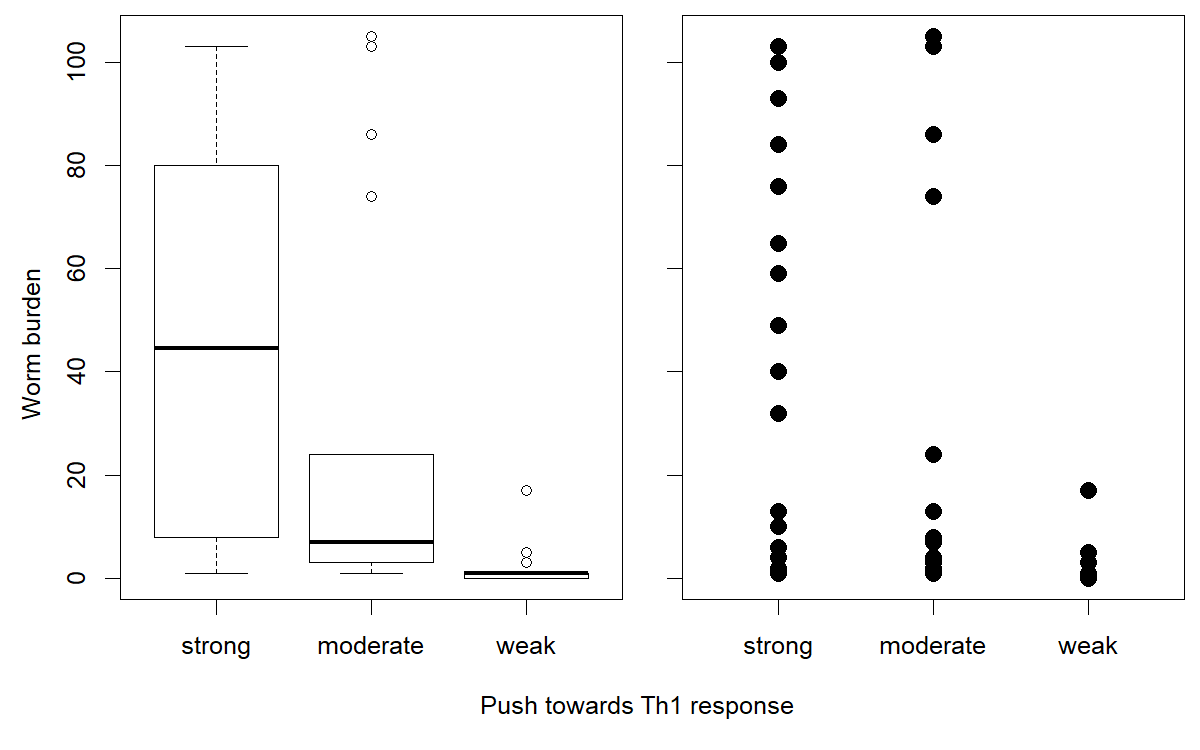
\includegraphics[width=\linewidth]{figure/unnamed-chunk-2-1} \hfill{}

\caption[There are many different ways to visualize this data]{There are many different ways to visualize this data. One possibility is to draw a constrast between the way immunological studies often represent data, which emphasizes mean differences between treatments, and a representation that emphasizes the variability among individuals within a treatment. Here I do that, representing treatments only in the non-specific way they were referenced in the datafile itself, in terms of the environmental push towards a Th1 (IFNg) response. That way of discussing treatment emphasizes that, as the push towards Th1 strengthens, so too does the worm burden.}\label{fig:unnamed-chunk-2}
\end{figure}


\end{knitrout}

\newpage

\begin{knitrout}\scriptsize
\definecolor{shadecolor}{rgb}{0.969, 0.969, 0.969}\color{fgcolor}\begin{figure}

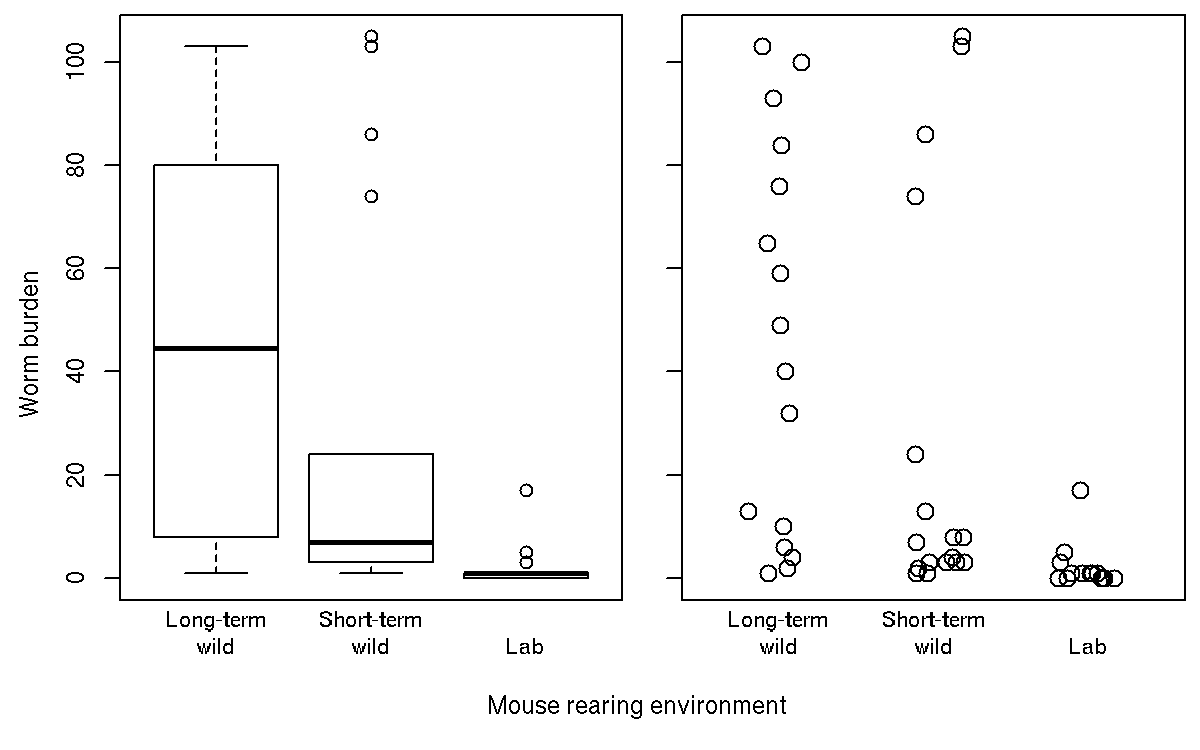
\includegraphics[width=\linewidth]{figure/unnamed-chunk-3-1} \hfill{}

\caption[However, there is also an argument that we should talk about this data in terms of the environmental treatments, since the Stony Ford aspect of this project is very important]{However, there is also an argument that we should talk about this data in terms of the environmental treatments, since the Stony Ford aspect of this project is very important. The left panel of this figure is essentially identical to Fig. 2 of Leung et al. 2018.}\label{fig:unnamed-chunk-3}
\end{figure}


\end{knitrout}

\newpage

\begin{knitrout}\scriptsize
\definecolor{shadecolor}{rgb}{0.969, 0.969, 0.969}\color{fgcolor}\begin{figure}

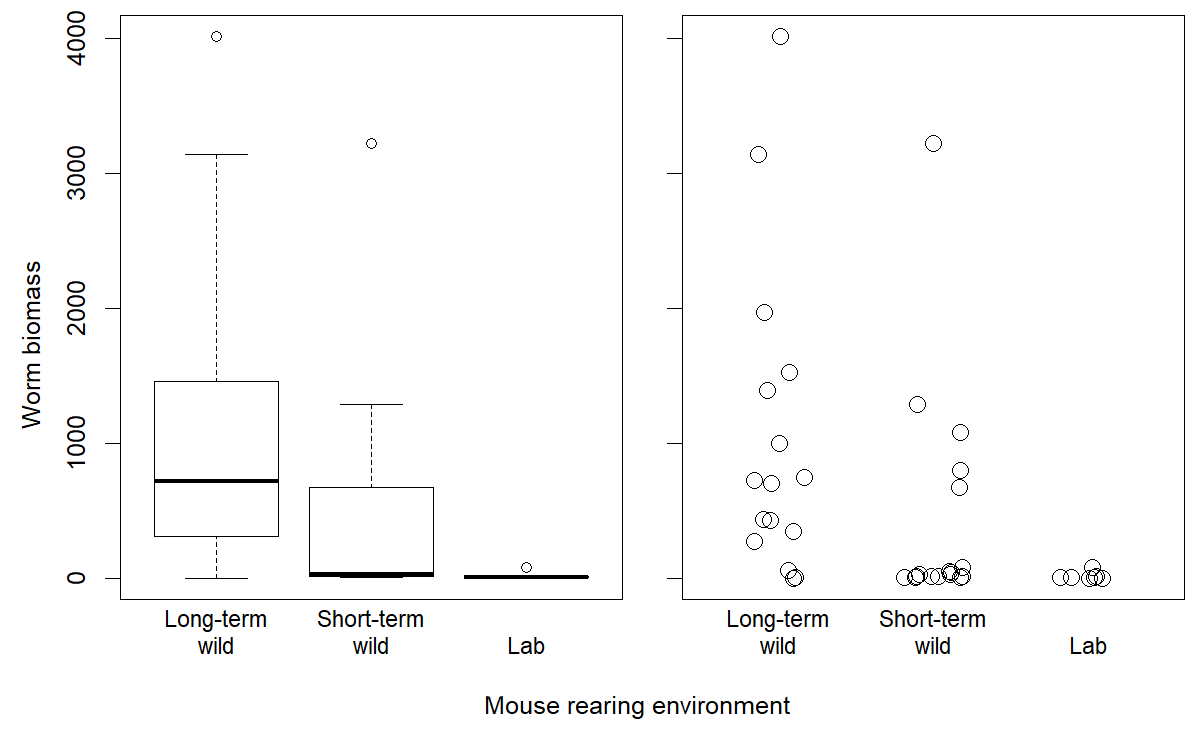
\includegraphics[width=\linewidth]{figure/unnamed-chunk-4-1} \hfill{}

\caption[This is very much like the preceding figure, except focused on worm biomass rather than worm burden]{This is very much like the preceding figure, except focused on worm biomass rather than worm burden.}\label{fig:unnamed-chunk-4}
\end{figure}


\end{knitrout}

\newpage

\begin{knitrout}\scriptsize
\definecolor{shadecolor}{rgb}{0.969, 0.969, 0.969}\color{fgcolor}\begin{figure}

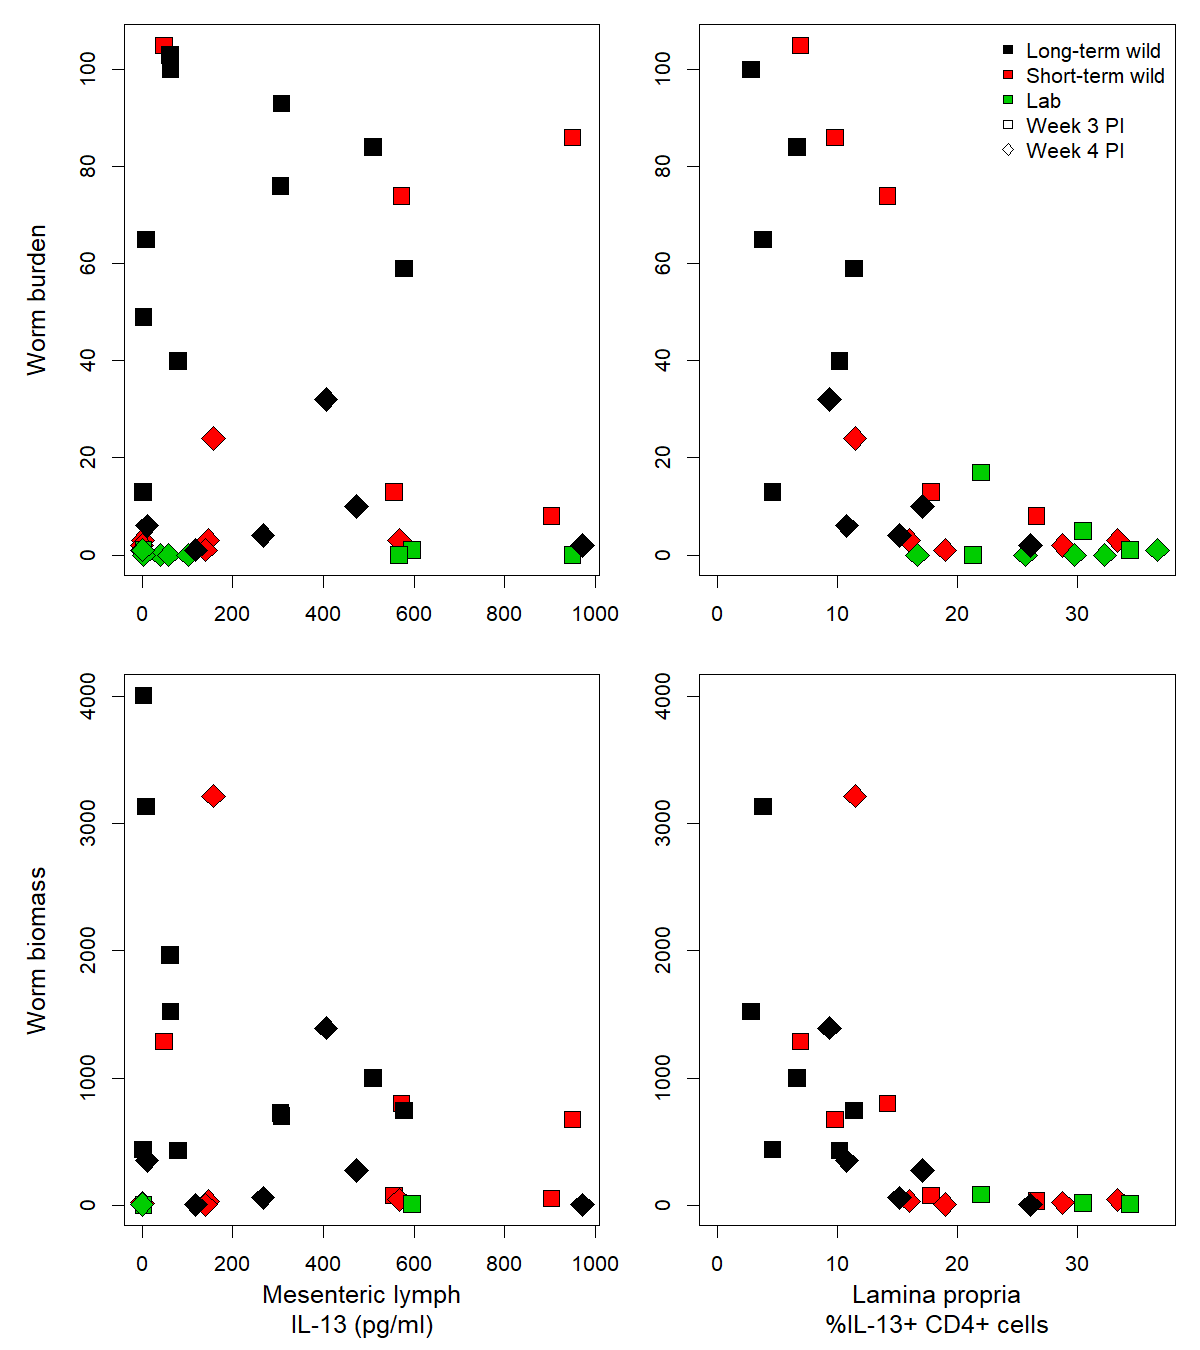
\includegraphics[width=\linewidth]{figure/unnamed-chunk-5-1} \hfill{}

\caption[Another thing that we want to show is that, across these environments, what predicts worm burden or biomass is actually that push towards Th1ness vs Th2ness]{Another thing that we want to show is that, across these environments, what predicts worm burden or biomass is actually that push towards Th1ness vs Th2ness. Here we can see that looking at the Th2 response in both the mesenteric lymph node and the lamina propria - the pattern is most obvious in the data from the lamina propria: the higher the fraction of CD4+ T-cells producing IL-13, the lower the worm burden, regardless of sampling date. In the lymph node, the relationship between total concentration of cytokine and worm burden is different at the different time points: at 3 weeks post-infection, high IL-13 is associated with low worm burden; at 4 weeks post-infection (when most individuals have cleared the infection (low worm burdens), the cytokine levels are much lower, likely reflecting reduced production of IL-13 due to the lower worm burden.}\label{fig:unnamed-chunk-5}
\end{figure}


\end{knitrout}

\newpage

\begin{knitrout}\scriptsize
\definecolor{shadecolor}{rgb}{0.969, 0.969, 0.969}\color{fgcolor}\begin{figure}

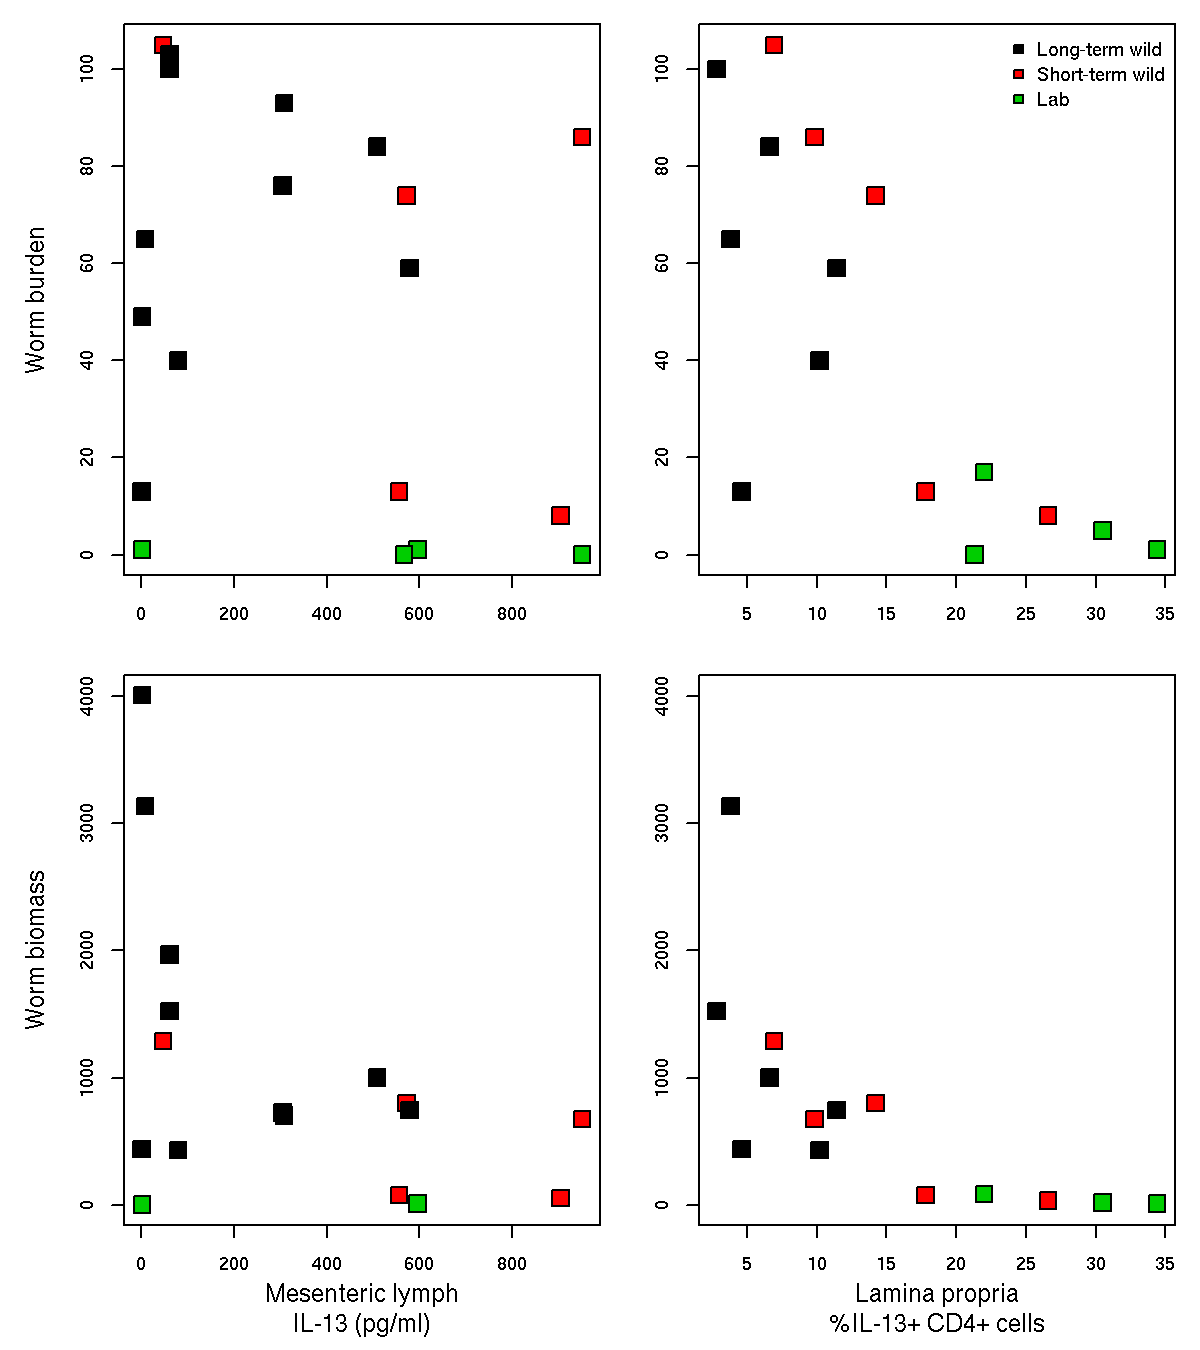
\includegraphics[width=\linewidth]{figure/unnamed-chunk-6-1} \hfill{}

\caption[This figure is identical to the preceding one, except that it only looks at the three-week data, which cleans up the resuls quite a lot]{This figure is identical to the preceding one, except that it only looks at the three-week data, which cleans up the resuls quite a lot. There are still some datapoints for the MLN data where individuals have low burdens and low IL-13, possibly because they are clearing the infection.}\label{fig:unnamed-chunk-6}
\end{figure}


\end{knitrout}


\newpage

\begin{knitrout}\scriptsize
\definecolor{shadecolor}{rgb}{0.969, 0.969, 0.969}\color{fgcolor}\begin{figure}

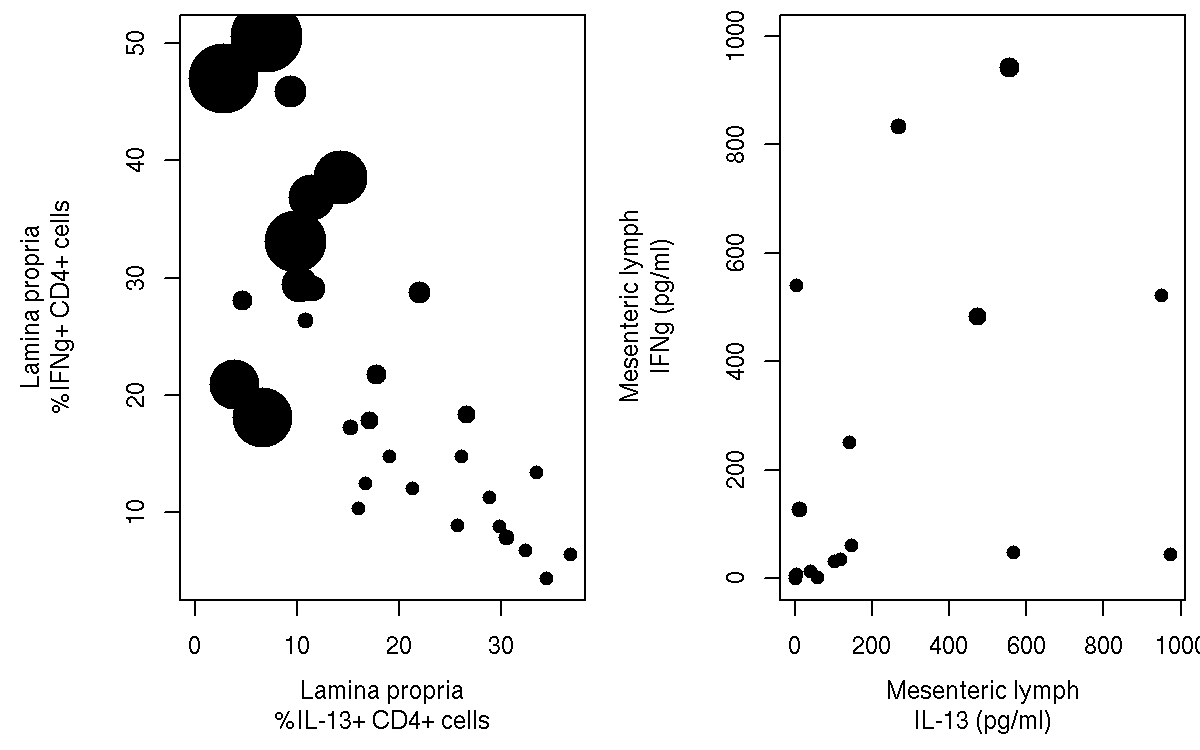
\includegraphics[width=\linewidth]{figure/unnamed-chunk-7-1} \hfill{}

\caption[Here we show that Th1ness and Th2ness are strongly negatively correlated with one another, in terms of the fraction of CD4+ T-cells expressing IL-13 versus IFNg]{Here we show that Th1ness and Th2ness are strongly negatively correlated with one another, in terms of the fraction of CD4+ T-cells expressing IL-13 versus IFNg. Point size in these figures is proportional to worm burden. It's hard to draw many conclusions from the data from the MLN - there are far fewer datapoints overall, and none of the datapoints came from animals with high worm burden.}\label{fig:unnamed-chunk-7}
\end{figure}


\end{knitrout}


\begin{knitrout}\scriptsize
\definecolor{shadecolor}{rgb}{0.969, 0.969, 0.969}\color{fgcolor}\begin{figure}

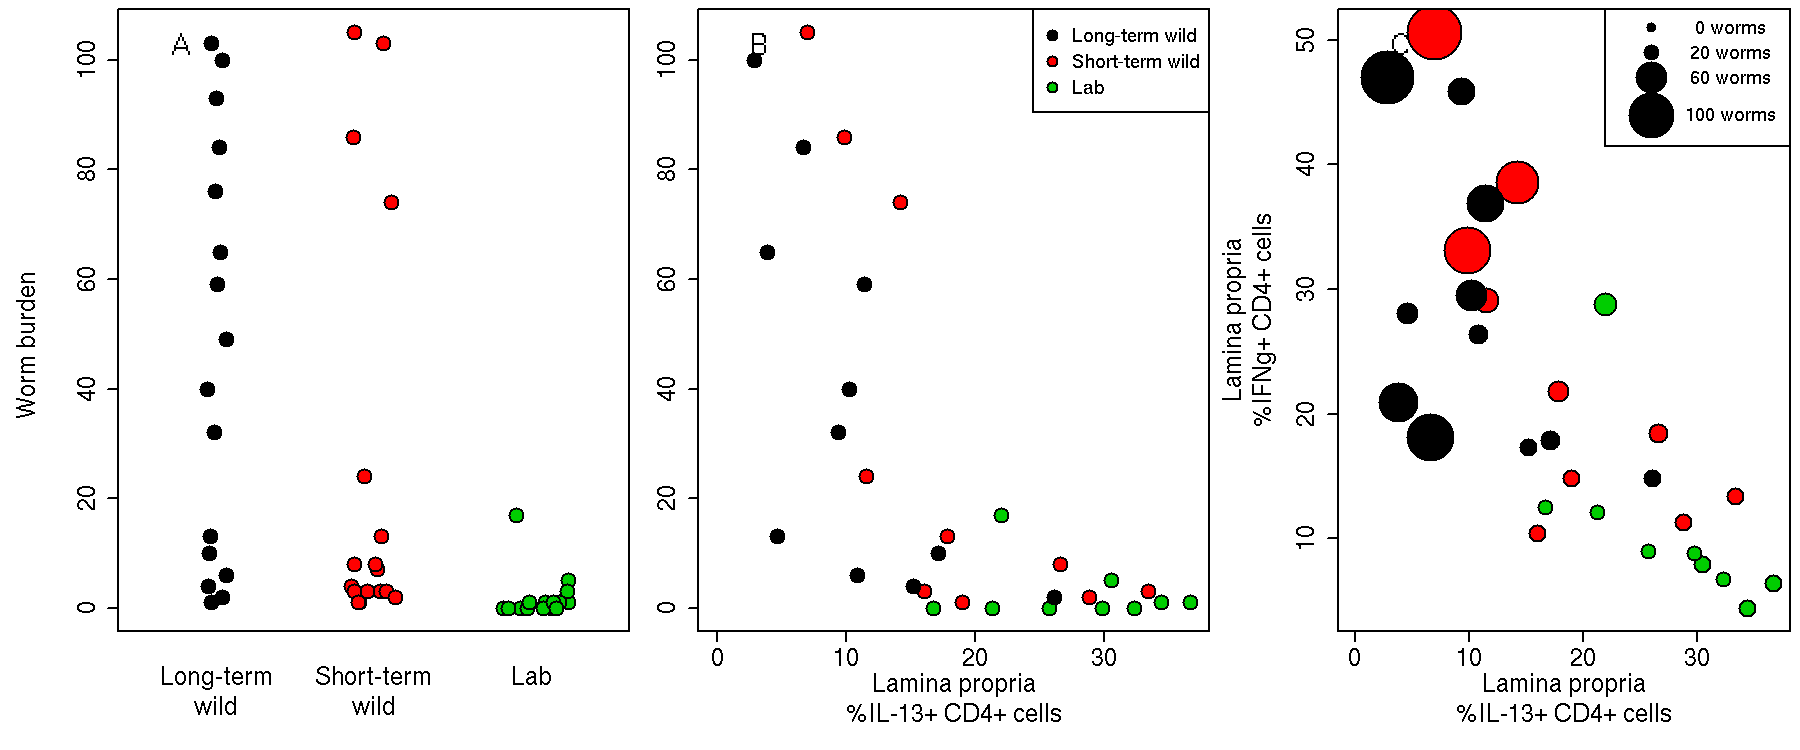
\includegraphics[width=\linewidth]{figure/unnamed-chunk-8-1} \hfill{}

\caption[(A) The rearing environment (lab versus wild) has a large effect on worm burden at 3- or 4-weeks post-infection]{(A) The rearing environment (lab versus wild) has a large effect on worm burden at 3- or 4-weeks post-infection. However, within treatments, there is considerable individual variation in worm burden. (B) Worm burden has a strong negative correlation with the fraction of CD4+ T-cells expressing Th2 cytokines, as expected. (C) Expression of Th2 cytokines by CD4+ T-cells is negatively correlated with expression of Th1 cytokines, further indicating that chronicity is determined by the immune-parasite battle over Th1-Th2 cytokine expression.}\label{fig:unnamed-chunk-8}
\end{figure}


\end{knitrout}




\end{document}
